%  LaTeX support: latex@mdpi.com 
%  For support, please attach all files needed for compiling as well as the log file, and specify your operating system, LaTeX version, and LaTeX editor.


%=================================================================
\documentclass[agriengineering,article,submit,pdftex,moreauthors]{Definitions/mdpi} 
%\documentclass[journal,article,submit,pdftex,moreauthors]{Definitions/mdpi} 


%\documentclass[preprints,article,submit,pdftex,moreauthors]{Definitions/mdpi} 
% For posting an early version of this manuscript as a preprint, you may use "preprints" as the journal. Changing "submit" to "accept" before posting will remove line numbers.

% Below journals will use APA reference format:
% admsci, behavsci, businesses, econometrics, economies, education, ejihpe, games, humans, ijfs, journalmedia, jrfm, languages, psycholint, publications, tourismhosp, youth

% Below journals will use Chicago reference format:
% arts, genealogy, histories, humanities, jintelligence, laws, literature, religions, risks, socsci

%--------------------
% Class Options:
%--------------------
%----------
% journal
%----------
% Choose between the following MDPI journals:
% accountaudit, acoustics, actuators, addictions, adhesives, admsci, adolescents, aerobiology, aerospace, agriculture, agriengineering, agrochemicals, agronomy, ai, air, algorithms, allergies, alloys, amh, analytica, analytics, anatomia, anesthres, animals, antibiotics, antibodies, antioxidants, applbiosci, appliedchem, appliedmath, appliedphys, applmech, applmicrobiol, applnano, applsci, aquacj, architecture, arm, arthropoda, arts, asc, asi, astronomy, atmosphere, atoms, audiolres, automation, axioms, bacteria, batteries, bdcc, behavsci, beverages, biochem, bioengineering, biologics, biology, biomass, biomechanics, biomed, biomedicines, biomedinformatics, biomimetics, biomolecules, biophysica, biosensors, biosphere, biotech, birds, blockchains, bloods, blsf, brainsci, breath, buildings, businesses, cancers, carbon, cardiogenetics, catalysts, cells, ceramics, challenges, chemengineering, chemistry, chemosensors, chemproc, children, chips, cimb, civileng, cleantechnol, climate, clinbioenerg, clinpract, clockssleep, cmd, cmtr, coasts, coatings, colloids, colorants, commodities, complications, compounds, computation, computers, condensedmatter, conservation, constrmater, cosmetics, covid, crops, cryo, cryptography, crystals, csmf, ctn, curroncol, cyber, dairy, data, ddc, dentistry, dermato, dermatopathology, designs, devices, diabetology, diagnostics, dietetics, digital, disabilities, diseases, diversity, dna, drones, dynamics, earth, ebj, ecm, ecologies, econometrics, economies, education, eesp, ejihpe, electricity, electrochem, electronicmat, electronics, encyclopedia, endocrines, energies, eng, engproc, ent, entomology, entropy, environments, epidemiologia, epigenomes, esa, est, famsci, fermentation, fibers, fintech, fire, fishes, fluids, foods, forecasting, forensicsci, forests, fossstud, foundations, fractalfract, fuels, future, futureinternet, futureparasites, futurepharmacol, futurephys, futuretransp, galaxies, games, gases, gastroent, gastrointestdisord, gastronomy, gels, genealogy, genes, geographies, geohazards, geomatics, geometry, geosciences, geotechnics, geriatrics, glacies, grasses, greenhealth, gucdd, hardware, hazardousmatters, healthcare, hearts, hemato, hematolrep, heritage, higheredu, highthroughput, histories, horticulturae, hospitals, humanities, humans, hydrobiology, hydrogen, hydrology, hygiene, idr, iic, ijerph, ijfs, ijgi, ijmd, ijms, ijns, ijpb, ijt, ijtm, ijtpp, ime, immuno, informatics, information, infrastructures, inorganics, insects, instruments, inventions, iot, j, jal, jcdd, jcm, jcp, jcs, jcto, jdad, jdb, jeta, jfb, jfmk, jimaging, jintelligence, jlpea, jmahp, jmmp, jmms, jmp, jmse, jne, jnt, jof, joitmc, joma, jop, jor, journalmedia, jox, jpbi, jpm, jrfm, jsan, jtaer, jvd, jzbg, kidney, kidneydial, kinasesphosphatases, knowledge, labmed, laboratories, land, languages, laws, life, lights, limnolrev, lipidology, liquids, literature, livers, logics, logistics, lubricants, lymphatics, machines, macromol, magnetism, magnetochemistry, make, marinedrugs, materials, materproc, mathematics, mca, measurements, medicina, medicines, medsci, membranes, merits, metabolites, metals, meteorology, methane, metrics, metrology, micro, microarrays, microbiolres, microelectronics, micromachines, microorganisms, microplastics, microwave, minerals, mining, mmphys, modelling, molbank, molecules, mps, msf, mti, multimedia, muscles, nanoenergyadv, nanomanufacturing, nanomaterials, ncrna, ndt, network, neuroglia, neurolint, neurosci, nitrogen, notspecified, nri, nursrep, nutraceuticals, nutrients, obesities, oceans, ohbm, onco, oncopathology, optics, oral, organics, organoids, osteology, oxygen, parasites, parasitologia, particles, pathogens, pathophysiology, pediatrrep, pets, pharmaceuticals, pharmaceutics, pharmacoepidemiology, pharmacy, philosophies, photochem, photonics, phycology, physchem, physics, physiologia, plants, plasma, platforms, pollutants, polymers, polysaccharides, populations, poultry, powders, preprints, proceedings, processes, prosthesis, proteomes, psf, psych, psychiatryint, psychoactives, psycholint, publications, purification, quantumrep, quaternary, qubs, radiation, reactions, realestate, receptors, recycling, regeneration, religions, remotesensing, reports, reprodmed, resources, rheumato, risks, robotics, rsee, ruminants, safety, sci, scipharm, sclerosis, seeds, sensors, separations, sexes, signals, sinusitis, siuj, skins, smartcities, sna, societies, socsci, software, soilsystems, solar, solids, spectroscj, sports, standards, stats, std, stresses, surfaces, surgeries, suschem, sustainability, symmetry, synbio, systems, tae, targets, taxonomy, technologies, telecom, test, textiles, thalassrep, therapeutics, thermo, timespace, tomography, tourismhosp, toxics, toxins, transplantology, transportation, traumacare, traumas, tropicalmed, universe, urbansci, uro, vaccines, vehicles, venereology, vetsci, vibration, virtualworlds, viruses, vision, waste, water, wem, wevj, wild, wind, women, world, youth, zoonoticdis

%---------
% article
%---------
% The default type of manuscript is "article", but can be replaced by: 
% abstract, addendum, article, benchmark, book, bookreview, briefcommunication, briefreport, casereport, changes, clinicopathologicalchallenge, comment, commentary, communication, conceptpaper, conferenceproceedings, correction, conferencereport, creative, datadescriptor, discussion, entry, expressionofconcern, extendedabstract, editorial, essay, erratum, fieldguide, hypothesis, interestingimages, letter, meetingreport, monograph, newbookreceived, obituary, opinion, proceedingpaper, projectreport, reply, retraction, review, perspective, protocol, shortnote, studyprotocol, supfile, systematicreview, technicalnote, viewpoint, guidelines, registeredreport, tutorial,  giantsinurology, urologyaroundtheworld
% supfile = supplementary materials

%----------
% submit
%----------
% The class option "submit" will be changed to "accept" by the Editorial Office when the paper is accepted. This will only make changes to the frontpage (e.g., the logo of the journal will get visible), the headings, and the copyright information. Also, line numbering will be removed. Journal info and pagination for accepted papers will also be assigned by the Editorial Office.

%------------------
% moreauthors
%------------------
% If there is only one author the class option oneauthor should be used. Otherwise use the class option moreauthors.

%---------
% pdftex
%---------
% The option pdftex is for use with pdfLaTeX. Remove "pdftex" for (1) compiling with LaTeX & dvi2pdf (if eps figures are used) or for (2) compiling with XeLaTeX.

%=================================================================
% MDPI internal commands - do not modify
\firstpage{1} 
\makeatletter 
\setcounter{page}{\@firstpage} 
\makeatother
\pubvolume{1}
\issuenum{1}
\articlenumber{0}
\pubyear{2025}
\copyrightyear{2024}
%\externaleditor{Firstname Lastname} % More than 1 editor, please add `` and '' before the last editor name
\datereceived{ } 
\daterevised{ } % Comment out if no revised date
\dateaccepted{ } 
\datepublished{ } 
%\datecorrected{} % For corrected papers: "Corrected: XXX" date in the original paper.
%\dateretracted{} % For retracted papers: "Retracted: XXX" date in the original paper.
\hreflink{https://doi.org/} % If needed use \linebreak
%\doinum{}
%\pdfoutput=1 % Uncommented for upload to arXiv.org
%\CorrStatement{yes}  % For updates
%\longauthorlist{yes} % For many authors that exceed the left citation part

%=================================================================
% Add packages and commands here. The following packages are loaded in our class file: fontenc, inputenc, calc, indentfirst, fancyhdr, graphicx, epstopdf, lastpage, ifthen, float, amsmath, amssymb, lineno, setspace, enumitem, mathpazo, booktabs, titlesec, etoolbox, tabto, xcolor, colortbl, soul, multirow, microtype, tikz, totcount, changepage, attrib, upgreek, array, tabularx, pbox, ragged2e, tocloft, marginnote, marginfix, enotez, amsthm, natbib, hyperref, cleveref, scrextend, url, geometry, newfloat, caption, draftwatermark, seqsplit
% cleveref: load \crefname definitions after \begin{document}

% BEM ADDITIONS BEGIN
\usepackage{longtable}
\usepackage{amsmath}

% BEM ADDITIONS END

%=================================================================
% Please use the following mathematics environments: Theorem, Lemma, Corollary, Proposition, Characterization, Property, Problem, Example, ExamplesandDefinitions, Hypothesis, Remark, Definition, Notation, Assumption
%% For proofs, please use the proof environment (the amsthm package is loaded by the MDPI class).

%=================================================================
% Full title of the paper (Capitalized)
\Title{Class Imbalance in Crop/Weed Classification}

% MDPI internal command: Title for citation in the left column
\TitleCitation{Class Imbalance in Crop/Weed Classification}

% Author Orchid ID: enter ID or remove command
\newcommand{\orcidauthorA}{0009-0002-3582-2576} % Add \orcidA{} behind the author's name
%\newcommand{\orcidauthorB}{0000-0000-0000-000X} % Add \orcidB{} behind the author's name

% Authors, for the paper (add full first names)
%\Author{Evan McGinnis $^{1,\dagger,\ddagger}$\orcidA{}, Firstname Lastname $^{2,\ddagger}$ and Firstname Lastname $^{2,}$*}
\Author{Brian E McGinnis $^{1,\dagger,\ddagger}$\orcidA{}}

%\longauthorlist{yes}

% MDPI internal command: Authors, for metadata in PDF
\AuthorNames{\orcidA Brian E McGinnis}

% MDPI internal command: Authors, for citation in the left column, only choose below one of them according to the journal style
% If this is a Chicago style journal: Lastname, Firstname, Firstname Lastname, and Firstname Lastname.
% If this is a APA style journal: Lastname, F., Lastname, F., \& Lastname, F.
% If this is a ACS style journal: Lastname, F.; Lastname, F.; Lastname, F.
%\isAPAStyle{%
%       \AuthorCitation{McGinnis, E., Lastname, F., \& Lastname, F.}
%         }{%
%        \isChicagoStyle{%
%        \AuthorCitation{McGinnis, E, Firstname Lastname, and Firstname Lastname.}
%        }{
%        \AuthorCitation{McGinnis, E.; Lastname, F.; Lastname, F.}
%        }
%}

\isAPAStyle{%
       \AuthorCitation{McGinnis, B.}
         }{%
        \isChicagoStyle{%
        \AuthorCitation{McGinnis, B}
        }{
        \AuthorCitation{McGinnis, B.}
        }
}

% Affiliations / Addresses (Add [1] after \address if there is only one affiliation.)
\address{%
$^{1}$ \quad Affiliation 1; evanmc@arizona.edu\\
}
%$^{2}$ \quad Affiliation 2; e-mail@e-mail.com}

% Contact information of the corresponding author
\corres{Correspondence: evanmc@arizona.edu}

% Current address and/or shared authorship
\firstnote{Current address: University of Arizona, Tucson, AZ 85721.}  % Current address should not be the same as any items in the Affiliation section.
\secondnote{These authors contributed equally to this work.}
% The commands \thirdnote{} till \eighthnote{} are available for further notes

%\simplesumm{} % Simple summary

%\conference{} % An extended version of a conference paper

% Abstract (Do not insert blank lines, i.e. \\) 
\abstract{This paper presents an overview of solutions to an all too common problem in the classification of vegetation in agricultural images: there are many more crop plants than there are weeds. There are two solutions to this problem examined in this paper: over-sampling the minority class and a combination of over-sampling the minority and under-sampling the majority. Oversampling the minority class involves the generation of synthetic data. Both approaches are evaluated in the context of the classification of crops and weeds. The analysis shows that these techniques improve KNN and SVM classification, improving the F1 scores achieved before and after imbalance correction.}

% Keywords
\keyword{imbalance, SMOTE, SVM, KNN, LDA, ENN, Tomek Links, over sampling} 

% The fields PACS, MSC, and JEL may be left empty or commented out if not applicable
%\PACS{J0101}
%\MSC{}
%\JEL{}

%%%%%%%%%%%%%%%%%%%%%%%%%%%%%%%%%%%%%%%%%%
% Only for the journal Diversity
%\LSID{\url{http://}}

%%%%%%%%%%%%%%%%%%%%%%%%%%%%%%%%%%%%%%%%%%
% Only for the journal Applied Sciences
%\featuredapplication{Authors are encouraged to provide a concise description of the specific application or a potential application of the work. This section is not mandatory.}
%%%%%%%%%%%%%%%%%%%%%%%%%%%%%%%%%%%%%%%%%%

%%%%%%%%%%%%%%%%%%%%%%%%%%%%%%%%%%%%%%%%%%
% Only for the journal Data
%\dataset{DOI number or link to the deposited data set if the data set is published separately. If the data set shall be published as a supplement to this paper, this field will be filled by the journal editors. In this case, please submit the data set as a supplement.}
%\datasetlicense{License under which the data set is made available (CC0, CC-BY, CC-BY-SA, CC-BY-NC, etc.)}

%%%%%%%%%%%%%%%%%%%%%%%%%%%%%%%%%%%%%%%%%%
% Only for the journal Toxins
%\keycontribution{The breakthroughs or highlights of the manuscript. Authors can write one or two sentences to describe the most important part of the paper.}

%%%%%%%%%%%%%%%%%%%%%%%%%%%%%%%%%%%%%%%%%%
% Only for the journal Encyclopedia
%\encyclopediadef{For entry manuscripts only: please provide a brief overview of the entry title instead of an abstract.}

%%%%%%%%%%%%%%%%%%%%%%%%%%%%%%%%%%%%%%%%%%
% Only for the journal Advances in Respiratory Medicine and Smart Cities
%\addhighlights{yes}
%\renewcommand{\addhighlights}{%

%\noindent This is an obligatory section in “Advances in Respiratory Medicine'' and ``Smart Cities”, whose goal is to increase the discoverability and readability of the article via search engines and other scholars. Highlights should not be a copy of the abstract, but a simple text allowing the reader to quickly and simplified find out what the article is about and what can be cited from it. Each of these parts should be devoted up to 2~bullet points.\vspace{3pt}\\
%\textbf{What are the main findings?}
% \begin{itemize}[labelsep=2.5mm,topsep=-3pt]
% \item First bullet.
% \item Second bullet.
% \end{itemize}\vspace{3pt}
%\textbf{What is the implication of the main finding?}
% \begin{itemize}[labelsep=2.5mm,topsep=-3pt]
% \item First bullet.
% \item Second bullet.
% \end{itemize}
%}

%%%%%%%%%%%%%%%%%%%%%%%%%%%%%%%%%%%%%%%%%%
\begin{document}

%%%%%%%%%%%%%%%%%%%%%%%%%%%%%%%%%%%%%%%%%%
%\setcounter{section}{-1} %% Remove this when starting to work on the template.
%\section{How to Use this Template}
%
%The template details the sections that can be used in a manuscript. Note that the order and names of article sections may differ from the requirements of the journal (e.g., the positioning of the Materials and Methods section). Please check the instructions on the authors' page of the journal to verify the correct order and names. For any questions, please contact the editorial office of the journal or support@mdpi.com. For LaTeX-related questions please contact latex@mdpi.com.%\endnote{This is an endnote.} % To use endnotes, please un-comment \printendnotes below (before References). Only journal Laws uses \footnote.

% The order of the section titles is different for some journals. Please refer to the "Instructions for Authors” on the journal homepage.




\section{Introduction}
Agricultural images of crops taken from an overhead perspective typically contain only two things: crop and weeds. While images taken from more than a meter above ground level (AGL) sometimes contain infrastructure equipment, and there may be other non-vegetative debris on the ground, crop and weed plants are the concern here. The application of a vegetation index to the image typically eliminates all non-vegetated elements of an images, leaving only the aforementioned plants. Imbalanced correction techniques are crucial for improving machine learning model performance when dealing with imbalanced datasets. Fortunately for the grower, but unfortunately for training classification models, these images often contain a much higher portion of crop than they do weeds, particularly if a pre-emergent herbicide has been applied or other active weed control measures are take. Having 10 weeds out of 100 plants in an image set might not be much of a problem, but having only three might be, especially taking into account a train/test split. The result may be that a weed is represented by only one or two samples. This paper focuses two general approaches to address this, generate new data for the minority class (over-sampling), and combine generation of new data and considering a subset of the majority class (under-sampling) This is where the term \textit{over-sampling} may lead readers to the wrong conclusion. The minority class is not over-sampled without modification simply by repeating the same data, but synthetic data is generated such that the ratio between the two classes does not exhibit an imbalance. The usual practice of segmenting the data into training and test portions has bearing on the procedures described. Only the training portion of the data is manipulated.

\section{Methodology}
Images were taken at the University of Arizona's Maricopa Agricultural Center (MAC) located in Maricopa, AZ of a cantaloupe planting in May 2024 (N 33.061813 W 111.965606). Images were obtained using an Apple iPhone 14, using ambient lighting. These images were color corrected using values obtained from images taken under identical lighting conditions of a Datacolor Spyder correction chart using Adobe Lightroom.  Images obtained using other sources are used to illustrate techniques or points, but most of the analysis shown in this document are from the set gathered at the MAC. All processing software was written in Python 3 and data analysis written in R.  The processing software depended heavily on three libraries: OpenCV (image processing), imbalanced-learn (imbalance correction), and scikit-learn (machine learning). The image sets examined were segmented using the Combined Indices 2 approach described by \citeauthor{Guerrero2012-zi} and manually assigned classification using software written by the author \cite{Guerrero2012-zi}.
Present in the image sets are two types of vegetation: crop and weeds. While the ratio of crop to weeds will most assuredly deviate from the 1:1 ideal, it is not particularly important what the specific ratio is, as the data will be trimmed to reflect the various ratios. That is, while a dataset may have a relatively low imbalance of 10:8, samples of the minority class are randomly discarded to achieve a much higher imbalance, say 50:1. Not covered in this breakdown, but quite important, is the topics of when to use imbalance correction techniques and when to perform parameter selection. This analysis will use a fairly commonly used train/test split of the data to form, and then test models. It is on this train set that the imbalance is corrected -- the objective is not to classify samples that are the result of correction, but to build a model that will produce results that exceed doing no correction. Parameter selection has similar concerns, but has some complications that merit mention here. Each plant in the image has color, texture, and shape attributes that are extracted and then the subset identified by PCA is used.\endnote{Details of the extracted features are beyond the scope of this document, but three features were identified as significant for each plant: GLCM dissimilarity average (shape), saturation (color), and solidity (shape).} The details of the extracted parameters is beyond the scope of this document, but what is not is when the parameter analysis takes place. Parameter analysis takes place prior to any imbalance correction.  As section \ref{section:over} details, new, synthetic entries can be constructed as part of imbalance correction, but the corrections are not considered in parameter selection, just the original data. That is, the parameters are selected from the training set prior to the generation of synthetic data for the minority class or removal of samples from the majority.

\section{Class Imbalance}
Plantings often exhibit a somewhat inconvenient feature: weeds and crop do not appear in the same proportion. While having a low weed count is probably desirable for crop production, it is not for classification when considering those images as a training set. While this can present itself as a relatively mild imbalance of nine weed plants for every 10 crop plants (certainly a bad situation for the grower) or a more extreme ratio of 1000 crop plants for every weed. In these extreme cases of imbalance, only a few samples of the minority class are used in classification if the overall size of the population is not particularly large -- and even more unfortunate case is that some weed species may not be present at all in the set used for training, as they are put into a testing class. \citeauthor{Fernandez2018-fw}, in a book discussing imbalanced datasets, detail several correction algorithms, among them SMOTE, ADASYN, Borderline SMOTE, kmeans, and SVM \cite{Fernandez2018-fw}. These algorithms seek to address the imbalance by the creation of synthetic samples of the minority class, correcting the class ratio to 1:1.  In most cases, of course, the solution is to simply collect sufficient data such that a severe imbalance does not exist, but this may not be a practical solution. This leaves two approaches: under-sample the majority or over-sample the minority. In cases where weeds (the minority) are relatively few, providing synthetic data to restore data to a 1:1 class ratio may be effective. There are various approaches that all have the same basic approach: generate data from the minority class that is similar -- but not identical -- to the data already present. That is, the minority class is effectively over-sampled, as elements of the minority class are used as the basis for new data.  Alternatively, the majority class can be under-sampled to achieve a 1:1 ratio, typically in two ways: randomly, and mathematical techniques that are more sensitive to the data relationships in the majority class.

\section{Over-Sampling}
\label{section:over}
Over-sampling is a bit more complex than the term implies -- minority samples are not simply sampled until the numbers are equal to a majority class. Just duplicating entries can correct the imbalance ratio back to the more desired 1:1, but does not add new data to the models being built than can be used to classify novel instances. Rather, new samples of the minority class are created, but the key question is \textit{which} of those minority instances form the basis of those synthetic samples? Are they chosen at random? Are they selected somehow?  In general, over-sampling tends to be preferred over under-sampling, as the latter may remove interesting data points from consideration. This question of which sample points in the minority set are used will be a topic revisited often as various techniques are described, as what points are used. Before details of various approaches are discussed, perhaps it is worthwhile to discuss why highly accurate predictions on highly imbalanced data are quite useless. Achieving a high accuracy in the case where the numbers of crop greatly outnumber the weeds is quite simple: predict everything is a crop. Consider a simplistic case of a dataset containing 100 crop plants and a single weed. Predicting each plant is a crop yields a model that is 99\% accurate, a satisfying, but useless, number.

 
\subsection{SMOTE}
The \textit{Synthetic Minority Oversampling TEchnique} is the basic technique used for re-balancing the data set -- other techniques in this section are extensions to that approach \cite{Chawla2002-dk}. Synthetic data is generated by selecting examples that are close in terms of the \textit{k} nearest neighbors, and selecting new points along the line connected those peers. This technique is not without drawbacks worthy of consideration: it generates data in the same direction, a complication for classification in that the decision surface is distorted, and tends to generate noisy data. The synthetic data points do not exhibit the same variation of the underlying real data points, leading to an introduction of over-fitting.
\begin{figure}[H]
	\centering
	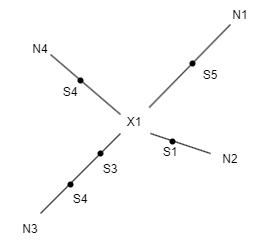
\includegraphics[scale=0.35]{./figures/smote.png}
	\caption[SMOTE selection of synthetic data points]{Generating synthetic data points using the SMOTE algorithm considers the \textit{k} nearest neighbors ($N_{1..4}$) to a point under consideration ($X_1$).  The SMOTE algorithm identifies points along the lines connecting a point to its neighbors ($S_{1..5}$). These points are the synthetic samples used to correct the imbalance.}
	\label{fig:smote}
\end{figure}

\subsection{ADASYN}
The Adaptive Synthetic Sampling approach considers the distribution of the minority points, giving more emphasis to points that a harder to learn. \cite{He2008-xr} Points that are harder to learn are those that are close to a class border, and in that sense, this approach is close to the \text{borderline} proposal. Contrast this with SMOTE. While sharing the same basic approach (considering the $k$ nearest neighbors), SMOTE samples the points uniformly, leading to an oversampling of dense areas, whereas ADASYN has no fixed ratio, but is based on learning difficulty. ADASYN will generate more points for these samples with high learning when processing the same dataset. The term \textit{harder to learn} is a bit imprecise, and warrants some further discussion. ADASYN creates as difficulty ratio for each point, representing the imbalance level in the local neighborhood of the point. This is done by comparing the number of majority class instances (non-minority) to the number of minority class instances within a specified radius around a point. Minority points with a large set of majority class neighbors are said to be harder to learn than those. A disadvantage of using ADASYN is that outlier points tend to have greater representation in the resulting dataset.


\subsection{Borderline}
In the standard SMOTE approach all members of the minority class are considered in synthetic data generation. In this variant first proposed by \citeauthor{Han2005-ui}, only those points far from the class border are considered. The rationale behind this approach is that points close to the border contribute little to distinguishing one class from the other, and should not form the basis for new data \cite{Han2005-ui}. In this scheme, points are considered noise if all of their neighbors are of the majority class. To be eligible for resampling, however, a point must have both majority and minority class neighbors. The rationale here is that samples close to a class border tend to be misclassified, and that by limiting the resampling to those points with the smallest risk of misclassification, the overall correct classification rate would be improved.
\begin{figure}[H]
	\centering
	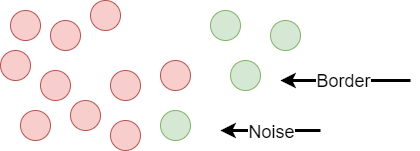
\includegraphics[scale=0.30]{./figures/borderline.png}
	\caption[Borderline selection of synthetic data points]{In the borderline variant of SMOTE, points close to the border having only majority class neighbors are considered noise, and are not considered as candidates for selection. }
	\label{fig:borderline}
\end{figure}



\subsection{KMeans}
This variant, like many of the others described here, addresses a weakness in basic SMOTE: points are selected randomly for oversampling consideration. A further downside of the base algorithm is the noise it introduces. This is not so much a SMOTE variant as it is a SMOTE supplement. As \citeauthor{Last2017-rh} states in a document introducing the algorithm:
\begin{quote}
\textit{
Another major concern is that SMOTE may further amplify noise present in the data. This is likely
to happen when linearly interpolating a noisy minority sample, which is located among majority class
instances, and its nearest minority neighbor. \cite{Last2017-rh}
}
\end{quote}
This approach differs from algorithms such as \textit{borderline} in that this approach views the class to be adjusted in terms of cluster membership.  In this approach, the clusters are formed with the \textit{kmeans} approach and SMOTE is applied to those clusters with a high portion of the minority class.

%
% This article seems to be available only for purchase as the library does not subscribe to that journal
% This is the reference both for borderline and SVM
%
\subsection{Support Vector Machine}
SVM SMOTE increases the points for the minority class along the decision boundary by generating new points along the lines connecting the support vectors and nearest neighbors \cite{Nguyen2011-cb}. In contrast with the KMeans approach, but in the same spirit as the borderline approach, this approach considers those points more important for estimating the best decision boundary, and therefor the best candidates for synthetic data generation. This approach first uses SMOTE to create new minority class samples and then uses the new minority class to train SVM. The samples that are identified as the most difficult to learn are then candidates for oversampling.

\section{Combined Under-sampling and Over-sampling}
\label{section:under}
Correcting the imbalance by under-sampling the majority class can have an unfortunate side-effect: information loss. Under-sampling, in its most basic form, involves discarding data to achieve the desired balance. Before the details of under-sampling are covered, perhaps this is a topic best addressed by a simple example. Consider the case where the majority class has 1000 samples, but only a few of those samples are representative without regard to the relationship between them (random discard), the discard may eliminate enough of those samples to have an appreciable effect when presented with a novel dataset. In weed/crop classification, however, members of the majority class (crop) are not likely to have small sets representative of a subset, especially if the sample set is taken from a single crop.
First proposed in 1976, \citeauthor{Tomek1976-bg} described a mechanism to choose discard samples based on their relationship to members of the minority class \cite{Tomek1976-bg}. Unlike the random selection of candidates, samples must have these characteristics to be considered a \textit{Tomek link}:
\begin{enumerate}
\item{Sample a’s nearest neighbor is b.}
\item{Sample b’s nearest neighbor is a.}
\item{Sample a and b belong to a different class.}
\end{enumerate}
Links with the lowest euclidean distance to  minority class are eliminated.
\begin{figure}[H]
	\centering
	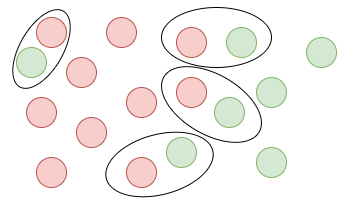
\includegraphics[scale=0.30]{./figures/tomek-a.png}
	\caption[Tomek links]{Tomek links are identified by the proximity of minority and majority class samples. Items with the lowest euclidean distance are eliminated.}
	\label{fig:tomek}
\end{figure}
A second common processing technique is using \textit{edited nearest neighbors} (ENN). The fundamental principle underlying ENN is to remove instances that differ from their nearest neighbors, with the assumption that such instances are likely to be mislabeled (differ from their neighbors) or noisy. The subsequent clarification of the decision boundary may contribute to better outcomes when the dataset is used for training.
\begin{enumerate}
\item{Compute the $k$ nearest neighbors for each observation in the dataset.}
\item{Compare the class label (crop or weed) of each instance with the class label of its $k$ nearest neighbors.}
\item{Remove instances from the majority class that differ from their neighbors}
\end{enumerate}

Typically, both under-sampling and oversampling techniques are used to address the imbalance, as \citeauthor{Batista2004-qz} describes \cite{Batista2004-qz}. 

\section{Results}

To assess the efficacy of over-sampling the minority and a combined over- and under-sampling approach, random instances in a dataset were first dropped to achieve five imbalance ratios and then restored to a 1:1 ratio between the two classes using the over-sampling techniques discussed. Models using the imbalanced data and the artificially balanced data were then compared in terms of the improvement (or degradation) of the Area Under the Curve (AUC) using nine different techniques: Random Forest, Extra Trees, Gradient Boosting, KNN, Linear Discriminant Analysis, Logistic Regression, Multi-Layer Perceptron, Random Forest, and Support Vector Machine. The Receiver Operating Characteristic (ROC) curve represents the probability that the model, if given a randomly chosen positive and negative example, will rank the positive higher than the negative. The AUC is the area underneath this curve -- the closer this area is to 1.0, the better a model is said to be.

As Figure \ref{fig:imbalance} shows, substituting synthetic data improves the AUC of various classification techniques in most cases, but some of the impact is quite trivial and -- in cases -- detrimental (note the case of using a \textit{Random Forest} approach to classification was almost always made worse by these approaches). 
%
% The imbalanced data and analysis requires 4 steps
%
%# 1) Copy the files to be analyzed
%# 2) Classify the vegetation automatically
%# 3) Correct the classifications manually
%# 4) Analyze for imbalance
%
% In post directory:
% make data-for-imbalance
% make classify-for-imbalance
% make review-for-imbalance
% This step should be run twice, 
% make analyze-imbalance INPUT=/cygdrive/d/maricopa-test/imbalance/processed/final/corrected.csv OUTPUT=imbalance.csv RATIO=30:5-10 STEPS=6 IMBALANCE=ALL-COMBINED
% make analyze-imbalance INPUT=/cygdrive/d/maricopa-test/imbalance/processed/final/corrected.csv OUTPUT=imbalance.csv RATIO=30:5-10 STEPS=6 IMBALANCE=ALL-OVER
%
% The actual analysis is performed by this command
% python ./imbalance.py -df ../jetson/training-from-dataframe.csv -ini ../jetson/standalone.ini -lg ../jetson/standalone-logging.ini -a ALL --classifier ALL
%
% The graph for the figure is created with the imbalanced.R script
% imbalance.R
%
\begin{figure}[H]
	\centering
	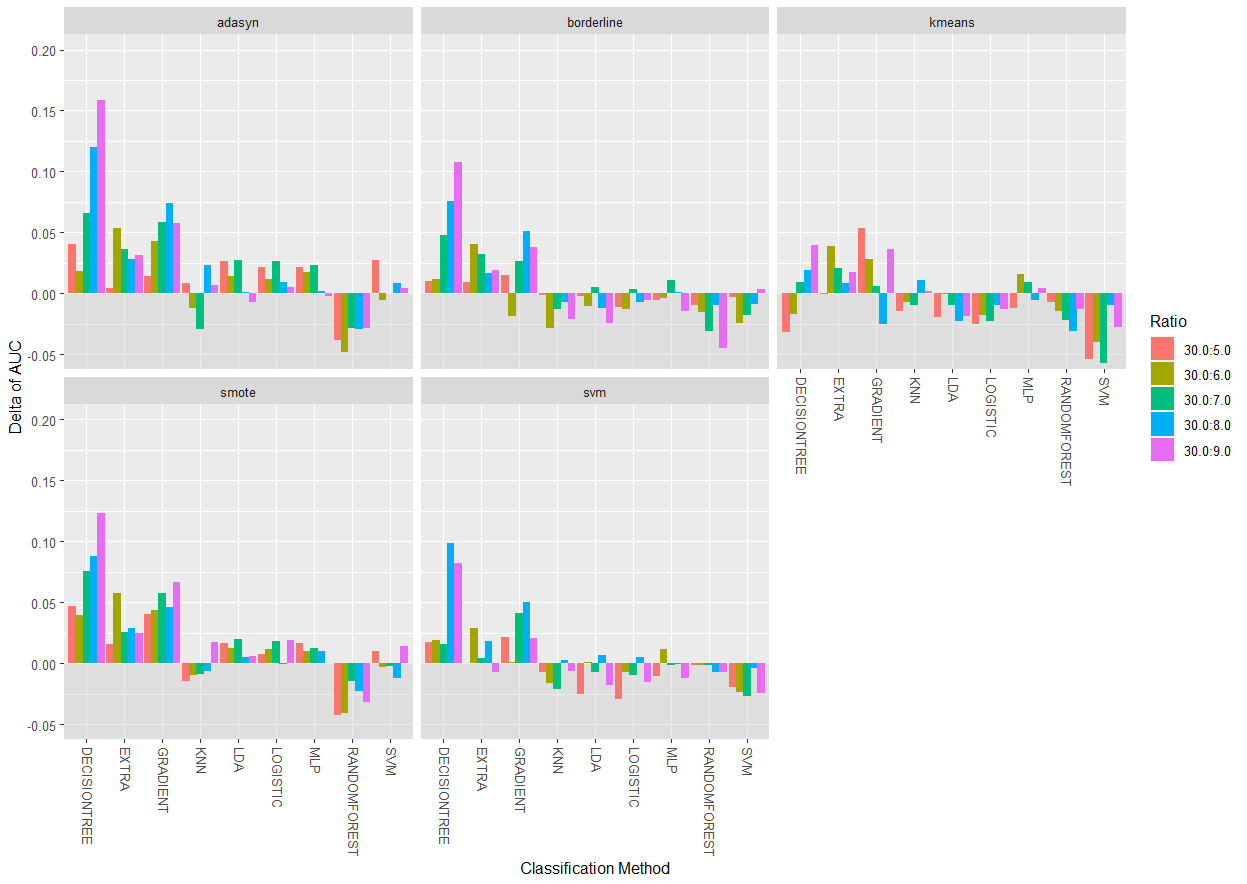
\includegraphics[width=0.9\linewidth]{./figures/imbalance.png}
	\caption[Class imbalance correction techniques]{The impact on AUC of class over-sampling imbalance correction techniques for various ratios and classification strategies can be seen in this visualization. Each facet of this display shows the effect of a different over-sampling technique. While many classification techniques are improved, the effect on Decision Tree classification is most pronounced. This dataset was first manipulated to achieve the desired ratio before the algorithms were applied. That is, to achieve a 30:1 imbalance, rows in the minority class were randomly dropped. The change in the AUC scores is shown in this plot for various ML techniques and for each of the correction approaches discussed.}
	\label{fig:imbalance}
\end{figure}

While the difference in the AUC achieved with classification using MLP and SVM (some clarification may be in order: SVM refers to a classification, and SVM-SMOTE refers to the correction technique.) stands out, almost all classification techniques were improved by the correction with a few exceptions. Correcting low-imbalance sets (30:5) yielded worse results in several instances. The postive impacts, however, can be characterized as minimal, however. Consider the ROC curves shown in Figure \ref{fig:auc}, showing the ROC curve achieved before and after correction using ADASYN.

\begin{figure*}[h]
	\centering
	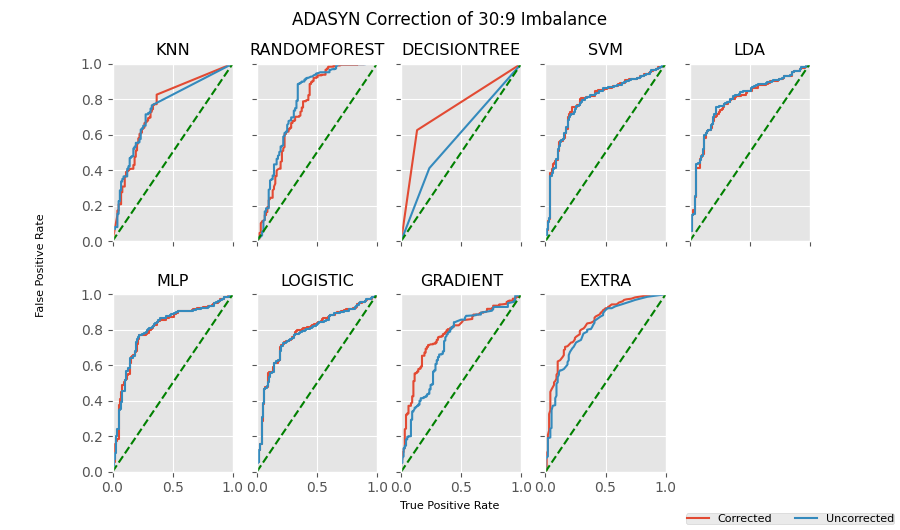
\includegraphics[height=0.25\textheight]{figures/roc-corrected.png}
	\caption[Before and after correction]{Before and after correction by oversampling the minority class with the ADASYN approach. Note that in many instances the effect of the correction on the ROC curve is quite modest. The dashed green line appearing in each of the graphs is representative of a random classifier, and appears only as a reference. A positive impact on classification using a gradient boosted technique is present, and that technique can certainly benefit from correction. }
	\label{fig:auc}
\end{figure*}

Combining over- and under-sampling techniques yielded worse results in many instances, but produced better results in most. As Figure \ref{fig:combined} shows, the impact tended to be more positive than negative.
\begin{figure}[H]
	\centering
	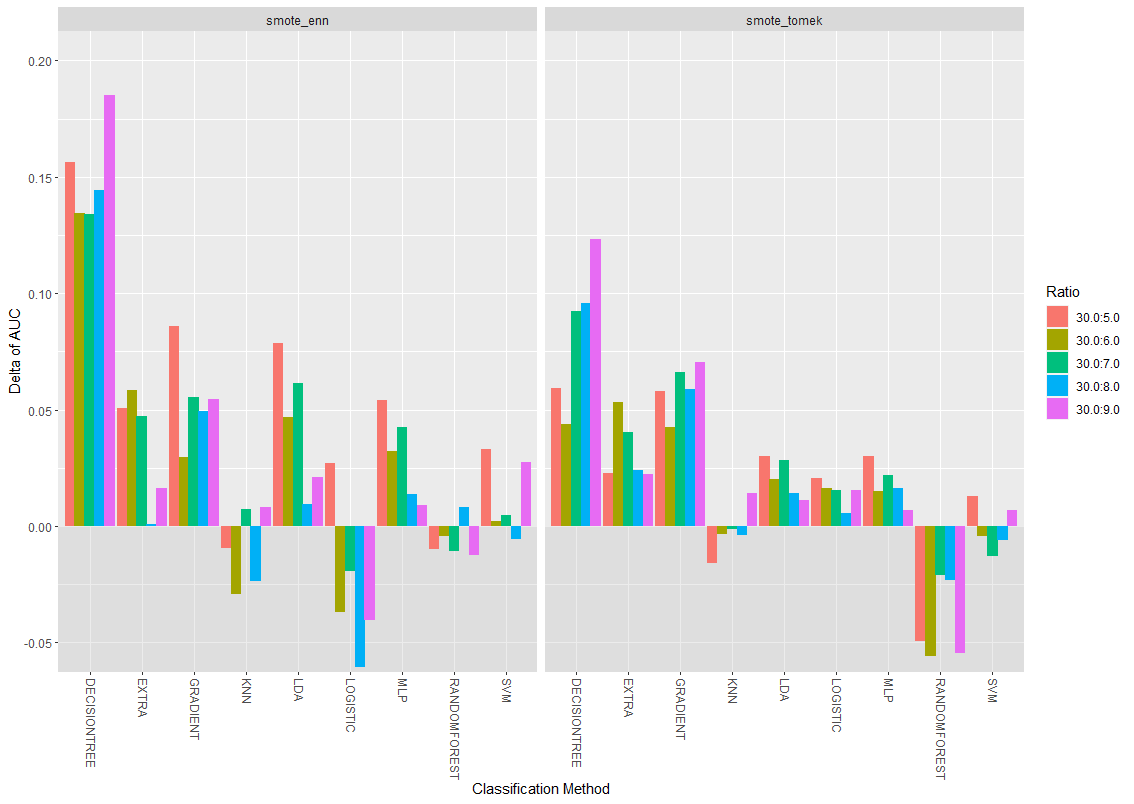
\includegraphics[width=0.9\linewidth]{./figures/combined.png}
	\caption[Combined Over and Under-sampling]{The impact on AUC of using a combined over- and under-sampling approach to class imbalance correction techniques for various ratios and classification strategies can be seen in this visualization. The strategy of using SMOTE+ENN has a particularly negative effect for many of the classification techniques, but the improvement in Decision Tree classification is a clear standout for both techniques.}
	\label{fig:combined}
\end{figure}

As with over-sampling the minority class, the effect was still modest, however. As seen in Figure \ref{fig:auc-tomek}, the ROC curves of uncorrected and corrected are, in general, quite close.  A notable exception was the difference in the curves shown by \textit{Gradient Boosting}. That classification technique visibly benefited from the combined approach of over- and under-sampling.

\begin{figure*}[h]
	\centering
	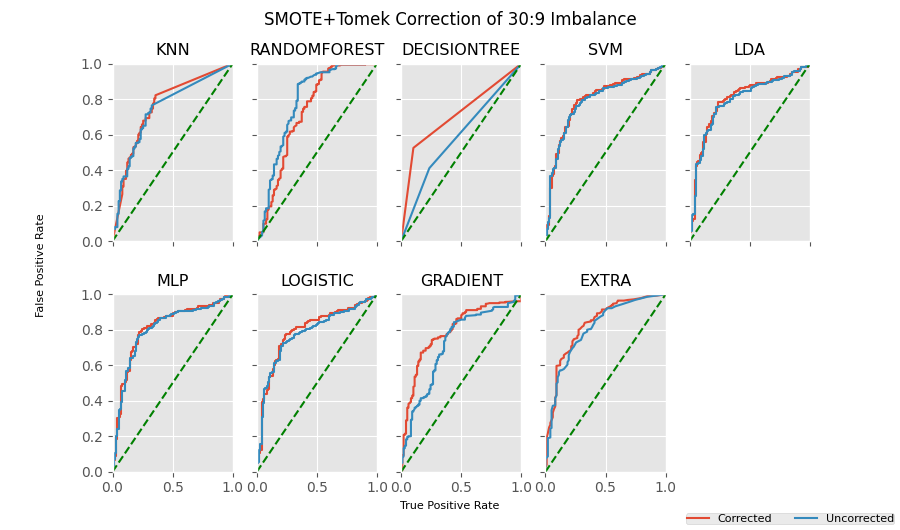
\includegraphics[height=0.25\textheight]{figures/roc-corrected-tomek.png}
	\caption[Before and after correction]{Before and after correction by a combined approach of over-sampling the minority class and under-sampling the majority class using Tomek links. Note that in many instances the effect of the correction is quite modest. A positive impact on classification using a gradient boosted technique is present, and that technique can certainly benefit from correction. }
	\label{fig:auc-tomek}
\end{figure*}

\section{Discussion}
Imbalance correction is not without cost, both computationally, and accuracy. Some classification techniques (Decision Tree, and SVM) are clear beneficiaries of correction, as both Figures \ref{fig:imbalance} \& \ref{fig:combined} show. Class imbalance correction is to overcome the bias seen in attempting to learn from situations where one class is significantly larger than another. Introducing a technique that does not improve this bias is not helpful; indeed its outcomes are worse in some situations. While the results reported here involve a single location (MAC) and on dates that were close together (late April and early May 2024), the findings warrant further investigation. Additionally, the correction implementation algorithms are not the product of the author \endnote{All processing was performed using the Python imbalanced-learn library that can be obtained from this website: https://imbalanced-learn.org/stable/\#}. While it is possible that errors in the implementation used affected the outcomes seen, the imbalance correction techniques examined in this research may not yield results that are acceptable for all situations. Indeed, for many of the techniques, the impact was quite modest overall, and the increase in accuracy may not be justified by the computational cost.




% Original MDPI Template Follows
%\subsection{Subsection}
%\subsubsection{Subsubsection}
%
%Bulleted lists look like this:
%\begin{itemize}
%\item	First bullet;
%\item	Second bullet;
%\item	Third bullet.
%\end{itemize}
%
%Numbered lists can be added as follows:
%\begin{enumerate}
%\item	First item; 
%\item	Second item;
%\item	Third item.
%\end{enumerate}
%
%The text continues here.
%
%\subsection{Figures, Tables and Schemes}
%
%All figures and tables should be cited in the main text as Figure~\ref{fig1}, Table~\ref{tab1}, etc.
%
%\begin{figure}[H]
%%\isPreprints{\centering}{} % Only used for preprints
%
\includegraphics[width=7 cm]{Definitions/logo-mdpi}
%\caption{This is a figure. Schemes follow the same formatting.\label{fig1}}
%\end{figure}   
%\unskip
%
%\begin{table}[H] 
%%\tablesize{\small}
%\caption{This is a table caption. Tables should be placed in the main text near to the first time they are~cited.\label{tab1}}
%%\isPreprints{\centering}{} % Only used for preprints
%\begin{tabularx}{\textwidth}{CCC}
%\toprule
%\textbf{Title 1}	& \textbf{Title 2}	& \textbf{Title 3}\\
%\midrule
%Entry 1		& Data			& Data\\
%Entry 2		& Data			& Data \textsuperscript{1}\\
%\bottomrule
%\end{tabularx}
%
%\noindent{\footnotesize{\textsuperscript{1} Tables may have a footer.}}
%\end{table}
%
%The text continues here (Figure~\ref{fig2} and Table~\ref{tab2}).
%
%% Example of a figure that spans the whole page width and with subfigures. The same concept works for tables, too.
%\begin{figure}[H]
%\centering
%%\isPreprints{}{% This command is only used for ``preprints''.
%\begin{adjustwidth}{-\extralength}{0cm}
%%} % If the paper is ``preprints'', please uncomment this parenthesis.
%\subfloat[\centering]{
\includegraphics[width=7.7cm]{Definitions/logo-mdpi}}
%\hfill
%\subfloat[\centering]{
\includegraphics[width=7.7cm]{Definitions/logo-mdpi}}\\
%\subfloat[\centering]{
\includegraphics[width=7.7cm]{Definitions/logo-mdpi}}
%\hfill
%\subfloat[\centering]{
\includegraphics[width=7.7cm]{Definitions/logo-mdpi}}
%%\isPreprints{}{% This command is only used for ``preprints''.
%\end{adjustwidth}
%%} % If the paper is ``preprints'', please uncomment this parenthesis.
%\caption{This is a wide figure. Schemes follow the same formatting. If there are multiple panels, they should be listed as: (\textbf{a}) Description of what is contained in the first panel. (\textbf{b}) Description of what is contained in the second panel. (\textbf{c}) Description of what is contained in the third panel. (\textbf{d}) Description of what is contained in the fourth panel. Figures should be placed in the main text near to the first time they are cited. A caption on a single line should be centered.\label{fig2}}
%\end{figure} 
%
%\begin{table}[H]
%\caption{This is a wide table.\label{tab2}}
%%\isPreprints{\centering}{% This command is only used for ``preprints''.
%	\begin{adjustwidth}{-\extralength}{0cm}
%%} % If the paper is ``preprints'', please uncomment this parenthesis.
%%\isPreprints{\begin{tabularx}{\textwidth}{CCCC}}{% This command is only used for ``preprints''.
%		\begin{tabularx}{\fulllength}{CCCC}
%%} % If the paper is ``preprints'', please uncomment this parenthesis.
%			\toprule
%			\textbf{Title 1}	& \textbf{Title 2}	& \textbf{Title 3}     & \textbf{Title 4}\\
%			\midrule
%\multirow[m]{3}{*}{Entry 1 *}	& Data			& Data			& Data\\
%			  	                   & Data			& Data			& Data\\
%			             	      & Data			& Data			& Data\\
%                   \midrule
%\multirow[m]{3}{*}{Entry 2}    & Data			& Data			& Data\\
%			  	                  & Data			& Data			& Data\\
%			             	     & Data			& Data			& Data\\
%			\bottomrule
%		\end{tabularx}
%%		\isPreprints{}{% This command is only used for ``preprints''.
%	\end{adjustwidth}
%%} % If the paper is ``preprints'', please uncomment this parenthesis.
%	\noindent{\footnotesize{* Tables may have a footer.}}
%\end{table}
%
%%\begin{listing}[H]
%%\caption{Title of the listing}
%%\rule{\columnwidth}{1pt}
%%\raggedright Text of the listing. In font size footnotesize, small, or normalsize. Preferred format: left aligned and single spaced. Preferred border format: top border line and bottom border line.
%%\rule{\columnwidth}{1pt}
%%\end{listing}
%
%Text.
%
%Text.
%
%\subsection{Formatting of Mathematical Components}
%
%This is the example 1 of equation:
%\begin{linenomath}
%\begin{equation}
%a = 1,
%\end{equation}
%\end{linenomath}
%the text following an equation need not be a new paragraph. Please punctuate equations as regular text.
%%% If the documentclass option "submit" is chosen, please insert a blank line before and after any math environment (equation and eqnarray environments). This ensures correct linenumbering. The blank line should be removed when the documentclass option is changed to "accept" because the text following an equation should not be a new paragraph.
%
%This is the example 2 of equation:
%%\isPreprints{}{% This command is only used for ``preprints''.
%\begin{adjustwidth}{-\extralength}{0cm}
%%} % If the paper is ``preprints'', please uncomment this parenthesis.
%\begin{equation}
%a = b + c + d + e + f + g + h + i + j + k + l + m + n + o + p + q + r + s + t + u + v + w + x + y + z
%\end{equation}
%%\isPreprints{}{% This command is only used for ``preprints''.
%\end{adjustwidth}
%%} % If the paper is ``preprints'', please uncomment this parenthesis.
%
%%% Example of a page in landscape format (with table and table footnote).
%%\startlandscape
%%\begin{table}[H] %% Table in wide page
%%%\isPreprints{\centering}{} % This command is only used for ``preprints''.
%%\caption{This is a very wide table.\label{tab3}}
%%	\begin{tabularx}{\textwidth}{CCCC}
%%		\toprule
%%		\textbf{Title 1}	& \textbf{Title 2}	& \textbf{Title 3}	& \textbf{Title 4}\\
%%		\midrule
%%		Entry 1		& Data			& Data			& This cell has some longer content that runs over two lines.\\
%%		Entry 2		& Data			& Data			& Data\textsuperscript{1}\\
%%		\bottomrule
%%	\end{tabularx}
%%%\isPreprints{}{% This command is only used for ``preprints''.
%%	\begin{adjustwidth}{+\extralength}{0cm}
%%%} % If the paper is ``preprints'', please uncomment this parenthesis.
%%		\noindent\footnotesize{\textsuperscript{1} This is a table footnote.}
%%%\isPreprints{}{% This command is only used for ``preprints''.
%%	\end{adjustwidth}
%%%} % If the paper is ``preprints'', please uncomment this parenthesis.
%%\end{table}
%%\finishlandscape
%
%
%Please punctuate equations as regular text. Theorem-type environments (including propositions, lemmas, corollaries etc.) can be formatted as follows:
%%% Example of a theorem:
%\begin{Theorem}
%Example text of a theorem.
%\end{Theorem}
%
%The text continues here. Proofs must be formatted as follows:
%
%%% Example of a proof:
%\begin{proof}[Proof of Theorem 1]
%Text of the proof. Note that the phrase ``of Theorem 1'' is optional if it is clear which theorem is being referred to.
%\end{proof}
%The text continues here.
%
%%%%%%%%%%%%%%%%%%%%%%%%%%%%%%%%%%%%%%%%%%%
%\section{Discussion}
%
%Authors should discuss the results and how they can be interpreted from the perspective of previous studies and of the working hypotheses. The findings and their implications should be discussed in the broadest context possible. Future research directions may also be highlighted.
%
%%%%%%%%%%%%%%%%%%%%%%%%%%%%%%%%%%%%%%%%%%%
%\section{Conclusions}
%
%This section is not mandatory, but can be added to the manuscript if the discussion is unusually long or complex.
%
%%%%%%%%%%%%%%%%%%%%%%%%%%%%%%%%%%%%%%%%%%%
%\section{Patents}
%
%This section is not mandatory, but may be added if there are patents resulting from the work reported in this manuscript.
%
%%%%%%%%%%%%%%%%%%%%%%%%%%%%%%%%%%%%%%%%%%%
%\vspace{6pt} 
%
%%%%%%%%%%%%%%%%%%%%%%%%%%%%%%%%%%%%%%%%%%%
%%% optional
%%\supplementary{The following supporting information can be downloaded at:  \linksupplementary{s1}, Figure S1: title; Table S1: title; Video S1: title.}
%
%% Only for journal Methods and Protocols:
%% If you wish to submit a video article, please do so with any other supplementary material.
%% \supplementary{The following supporting information can be downloaded at: \linksupplementary{s1}, Figure S1: title; Table S1: title; Video S1: title. A supporting video article is available at doi: link.}
%
%% Only used for preprtints:
%% \supplementary{The following supporting information can be downloaded at the website of this paper posted on \href{https://www.preprints.org/}{Preprints.org}.}
%
%% Only for journal Hardware:
%% If you wish to submit a video article, please do so with any other supplementary material.
%% \supplementary{The following supporting information can be downloaded at: \linksupplementary{s1}, Figure S1: title; Table S1: title; Video S1: title.\vspace{6pt}\\
%%\begin{tabularx}{\textwidth}{lll}
%%\toprule
%%\textbf{Name} & \textbf{Type} & \textbf{Description} \\
%%\midrule
%%S1 & Python script (.py) & Script of python source code used in XX \\
%%S2 & Text (.txt) & Script of modelling code used to make Figure X \\
%%S3 & Text (.txt) & Raw data from experiment X \\
%%S4 & Video (.mp4) & Video demonstrating the hardware in use \\
%%... & ... & ... \\
%%\bottomrule
%%\end{tabularx}
%%}
%
%%%%%%%%%%%%%%%%%%%%%%%%%%%%%%%%%%%%%%%%%%%
% BEM -- not applicable
%\authorcontributions{For research articles with several authors, a short paragraph specifying their individual contributions must be provided. The following statements should be used ``Conceptualization, X.X. and Y.Y.; methodology, X.X.; software, X.X.; validation, X.X., Y.Y. and Z.Z.; formal analysis, X.X.; investigation, X.X.; resources, X.X.; data curation, X.X.; writing---original draft preparation, X.X.; writing---review and editing, X.X.; visualization, X.X.; supervision, X.X.; project administration, X.X.; funding acquisition, Y.Y. All authors have read and agreed to the published version of the manuscript.'', please turn to the  \href{http://img.mdpi.org/data/contributor-role-instruction.pdf}{CRediT taxonomy} for the term explanation. Authorship must be limited to those who have contributed substantially to the work~reported.}

\funding{This research received no external funding.}

%\institutionalreview{In this section, you should add the Institutional Review Board Statement and approval number, if relevant to your study. You might choose to exclude this statement if the study did not require ethical approval. Please note that the Editorial Office might ask you for further information. Please add “The study was conducted in accordance with the Declaration of Helsinki, and approved by the Institutional Review Board (or Ethics Committee) of NAME OF INSTITUTE (protocol code XXX and date of approval).” for studies involving humans. OR “The animal study protocol was approved by the Institutional Review Board (or Ethics Committee) of NAME OF INSTITUTE (protocol code XXX and date of approval).” for studies involving animals. OR “Ethical review and approval were waived for this study due to REASON (please provide a detailed justification).” OR “Not applicable” for studies not involving humans or animals.}

%\informedconsent{Any research article describing a study involving humans should contain this statement. Please add ``Informed consent was obtained from all subjects involved in the study.'' OR ``Patient consent was waived due to REASON (please provide a detailed justification).'' OR ``Not applicable'' for studies not involving humans. You might also choose to exclude this statement if the study did not involve humans.

%Written informed consent for publication must be obtained from participating patients who can be identified (including by the patients themselves). Please state ``Written informed consent has been obtained from the patient(s) to publish this paper'' if applicable.}

\dataavailability{All code used in the preparation of this paper is available from \href{https://github.com/evan-mcginnis/imbalance}{GitHub}. Raw data is available from \href{https://doi.org/10.6084/m9.figshare.28147181}{Figshare}.} 

% Only for journal Drones
%\durcstatement{Current research is limited to the [please insert a specific academic field, e.g., XXX], which is beneficial [share benefits and/or primary use] and does not pose a threat to public health or national security. Authors acknowledge the dual-use potential of the research involving xxx and confirm that all necessary precautions have been taken to prevent potential misuse. As an ethical responsibility, authors strictly adhere to relevant national and international laws about DURC. Authors advocate for responsible deployment, ethical considerations, regulatory compliance, and transparent reporting to mitigate misuse risks and foster beneficial outcomes.}

% Only for journal Nursing Reports
%\publicinvolvement{Please describe how the public (patients, consumers, carers) were involved in the research. Consider reporting against the GRIPP2 (Guidance for Reporting Involvement of Patients and the Public) checklist. If the public were not involved in any aspect of the research add: ``No public involvement in any aspect of this research''.}
%
%% Only for journal Nursing Reports
%\guidelinesstandards{Please add a statement indicating which reporting guideline was used when drafting the report. For example, ``This manuscript was drafted against the XXX (the full name of reporting guidelines and citation) for XXX (type of research) research''. A complete list of reporting guidelines can be accessed via the equator network: \url{https://www.equator-network.org/}.}
%
%% Only for journal Nursing Reports
%\useofartificialintelligence{Please describe in detail any and all uses of artificial intelligence (AI) or AI-assisted tools used in the preparation of the manuscript. This may include, but is not limited to, language translation, language editing and grammar, or generating text. Alternatively, please state that “AI or AI-assisted tools were not used in drafting any aspect of this manuscript”.}

\acknowledgments{Thanks to Drs. Diaa Elshika and Said Atallah of the University of Arizona for access to the fields where images were acquired.}

\conflictsofinterest{None.} 

%%%%%%%%%%%%%%%%%%%%%%%%%%%%%%%%%%%%%%%%%%
%% Optional

%% Only for journal Encyclopedia
%\entrylink{The Link to this entry published on the encyclopedia platform.}

%
% BEM -- all terms should be defined in text -- not needed
%\abbreviations{Abbreviations}{
%The following abbreviations are used in this manuscript:\\
%
%\noindent 
%\begin{tabular}{@{}ll}
%MDPI & Multidisciplinary Digital Publishing Institute\\
%DOAJ & Directory of open access journals\\
%TLA & Three letter acronym\\
%LD & Linear dichroism
%\end{tabular}
%}

%%%%%%%%%%%%%%%%%%%%%%%%%%%%%%%%%%%%%%%%%%
%% Optional
%% BEM -- not needed 
%%\appendixtitles{no} % Leave argument "no" if all appendix headings stay EMPTY (then no dot is printed after "Appendix A"). If the appendix sections contain a heading then change the argument to "yes".
%%\appendixstart
%%\appendix
%%\section[\appendixname~\thesection]{}
%%\subsection[\appendixname~\thesubsection]{}
%%The appendix is an optional section that can contain details and data supplemental to the main text---for example, explanations of experimental details that would disrupt the flow of the main text but nonetheless remain crucial to understanding and reproducing the research shown; figures of replicates for experiments of which representative data are shown in the main text can be added here if brief, or as Supplementary Data. Mathematical proofs of results not central to the paper can be added as an appendix.
%%
%%\begin{table}[H] 
%%\caption{This is a table caption.\label{tab5}}
%%%\newcolumntype{C}{>{\centering\arraybackslash}X}
%%\begin{tabularx}{\textwidth}{CCC}
%%\toprule
%%\textbf{Title 1}	& \textbf{Title 2}	& \textbf{Title 3}\\
%%\midrule
%%Entry 1		& Data			& Data\\
%%Entry 2		& Data			& Data\\
%%\bottomrule
%%\end{tabularx}
%%\end{table}
%%
%%\section[\appendixname~\thesection]{}
%%All appendix sections must be cited in the main text. In the appendices, Figures, Tables, etc. should be labeled, starting with ``A''---e.g., Figure A1, Figure A2, etc.

%%%%%%%%%%%%%%%%%%%%%%%%%%%%%%%%%%%%%%%%%%
%\isPreprints{} % If the paper is ``preprints'', please uncomment this parenthesis.
\printendnotes[custom] % Un-comment to print a list of endnotes

\reftitle{References}

% Please provide either the correct journal abbreviation (e.g. according to the “List of Title Word Abbreviations” http://www.issn.org/services/online-services/access-to-the-ltwa/) or the full name of the journal.
% Citations and References in Supplementary files are permitted provided that they also appear in the reference list here. 

%=====================================
% References, variant A: external bibliography
%=====================================
\bibliography{../paperpile.bib}

%=====================================
% References, variant B: internal bibliography
%=====================================

%% ACS format
%\isAPAandChicago{}{%
%\begin{thebibliography}{999}
%% Reference 1
%\bibitem[Author1(year)]{ref-journal}
%Author~1, T. The title of the cited article. {\em Journal Abbreviation} {\bf 2008}, {\em 10}, 142--149.
%% Reference 2
%\bibitem[Author2(year)]{ref-book1}
%Author~2, L. The title of the cited contribution. In {\em The Book Title}; Editor 1, F., Editor 2, A., Eds.; Publishing House: City, Country, 2007; pp. 32--58.
%% Reference 3
%\bibitem[Author1 and Author2 (year)]{ref-book2}
%Author 1, A.; Author 2, B. \textit{Book Title}, 3rd ed.; Publisher: Publisher Location, Country, 2008; pp. 154--196.
%% Reference 4
%\bibitem[Author4(year)]{ref-unpublish}
%Author 1, A.B.; Author 2, C. Title of Unpublished Work. \textit{Abbreviated Journal Name} year, \textit{phrase indicating stage of publication (submitted; accepted; in press)}.
%% Reference 5
%\bibitem[Author8(year)]{ref-url}
%Title of Site. Available online: URL (accessed on Day Month Year).
%% Reference 6
%\bibitem[Author6(year)]{ref-proceeding}
%Author 1, A.B.; Author 2, C.D.; Author 3, E.F. Title of presentation. In Proceedings of the Name of the Conference, Location of Conference, Country, Date of Conference (Day Month Year); Abstract Number (optional), Pagination (optional).
%% Reference 7
%\bibitem[Author7(year)]{ref-thesis}
%Author 1, A.B. Title of Thesis. Level of Thesis, Degree-Granting University, Location of University, Date of Completion.
%\end{thebibliography}
%}
%
%% Chicago format (Used for journal: arts, genealogy, histories, humanities, jintelligence, laws, literature, religions, risks, socsci)
%\isChicagoStyle{%
%\begin{thebibliography}{999}
%% Reference 1
%\bibitem[Aranceta-Bartrina(1999a)]{ref-journal}
%Aranceta-Bartrina, Javier. 1999a. Title of the cited article. \textit{Journal Title} 6: 100--10.
%% Reference 2
%\bibitem[Aranceta-Bartrina(1999b)]{ref-book1}
%Aranceta-Bartrina, Javier. 1999b. Title of the chapter. In \textit{Book Title}, 2nd ed. Edited by Editor 1 and Editor 2. Publication place: Publisher, vol. 3, pp. 54–96.
%% Reference 3
%\bibitem[Baranwal and Munteanu {[1921]}(1955)]{ref-book2}
%Baranwal, Ajay K., and Costea Munteanu. 1955. \textit{Book Title}. Publication place: Publisher, pp. 154--96. First published 1921 (op-tional).
%% Reference 4
%\bibitem[Berry and Smith(1999)]{ref-thesis}
%Berry, Evan, and Amy M. Smith. 1999. Title of Thesis. Level of Thesis, Degree-Granting University, City, Country. Identifi-cation information (if available).
%% Reference 5
%\bibitem[Cojocaru et al.(1999)]{ref-unpublish}
%Cojocaru, Ludmila, Dragos Constatin Sanda, and Eun Kyeong Yun. 1999. Title of Unpublished Work. \textit{Journal Title}, phrase indicating stage of publication.
%% Reference 6
%\bibitem[Driver et al.(2000)]{ref-proceeding}
%Driver, John P., Steffen Rohrs, and Sean Meighoo. 2000. Title of Presentation. In \textit{Title of the Collected Work} (if available). Paper presented at Name of the Conference, Location of Conference, Date of Conference.
%% Reference 7
%\bibitem[Harwood(2008)]{ref-url}
%Harwood, John. 2008. Title of the cited article. Available online: URL (accessed on Day Month Year).
%\end{thebibliography}
%}{}
%
%% APA format (Used for journal: admsci, behavsci, businesses, econometrics, economies, education, ejihpe, games, humans, ijfs, journalmedia, jrfm, languages, psycholint, publications, tourismhosp, youth)
%\isAPAStyle{%
%\begin{thebibliography}{999}
%% Reference 1
%\bibitem[\protect\citeauthoryear{Azikiwe \BBA\ Bello}{{2020a}}]{ref-journal}
%Azikiwe, H., \& Bello, A. (2020a). Title of the cited article. \textit{Journal Title}, \textit{Volume}(Issue), 
%Firstpage--Lastpage/Article Number.
%% Reference 2
%\bibitem[\protect\citeauthoryear{Azikiwe \BBA\ Bello}{{2020b}}]{ref-book1}
%Azikiwe, H., \& Bello, A. (2020b). \textit{Book title}. Publisher Name.
%% Reference 3
%\bibitem[Davison(1623/2019)]{ref-book2}
%Davison, T. E. (2019). Title of the book chapter. In A. A. Editor (Ed.), \textit{Title of the book: Subtitle} 
%(pp. Firstpage--Lastpage). Publisher Name. (Original work published 1623) (Optional).
%% Reference 4
%\bibitem[Fistek et al.(2017)]{ref-proceeding}
%Fistek, A., Jester, E., \& Sonnenberg, K. (2017, Month Day). Title of contribution [Type of contribution]. Conference Name, Conference City, Conference Country.
%% Reference 5
%\bibitem[Hutcheson(2012)]{ref-thesis}
%Hutcheson, V. H. (2012). \textit{Title of the thesis} [XX Thesis, Name of Institution Awarding the Degree].
%% Reference 6
%\bibitem[Lippincott \& Poindexter(2019)]{ref-unpublish}
%Lippincott, T., \& Poindexter, E. K. (2019). \textit{Title of the unpublished manuscript} [Unpublished manuscript/Manuscript in prepara-tion/Manuscript submitted for publication]. Department Name, Institution Name.
%% Reference 7
%\bibitem[Harwood(2008)]{ref-url}
%Harwood, J. (2008). \textit{Title of the cited article}. Available online: URL (accessed on Day Month Year).
%\end{thebibliography}
%}{}

% If authors have biography, please use the format below
%\section*{Short Biography of Authors}
%\bio
%{\raisebox{-0.35cm}{\includegraphics[width=3.5cm,height=5.3cm,clip,keepaspectratio]{Definitions/author1.pdf}}}
%{\textbf{Firstname Lastname} Biography of first author}
%
%\bio
%{\raisebox{-0.35cm}{\includegraphics[width=3.5cm,height=5.3cm,clip,keepaspectratio]{Definitions/author2.jpg}}}
%{\textbf{Firstname Lastname} Biography of second author}

% For the MDPI journals use author-date citation, please follow the formatting guidelines on http://www.mdpi.com/authors/references
% To cite two works by the same author: \citeauthor{ref-journal-1a} (\citeyear{ref-journal-1a}, \citeyear{ref-journal-1b}). This produces: Whittaker (1967, 1975)
% To cite two works by the same author with specific pages: \citeauthor{ref-journal-3a} (\citeyear{ref-journal-3a}, p. 328; \citeyear{ref-journal-3b}, p.475). This produces: Wong (1999, p. 328; 2000, p. 475)

%%%%%%%%%%%%%%%%%%%%%%%%%%%%%%%%%%%%%%%%%%
%% for journal Sci
%\reviewreports{\\
%Reviewer 1 comments and authors’ response\\
%Reviewer 2 comments and authors’ response\\
%Reviewer 3 comments and authors’ response
%}
%%%%%%%%%%%%%%%%%%%%%%%%%%%%%%%%%%%%%%%%%%
\PublishersNote{}
%\isPreprints{} % If the paper is ``preprints'', please uncomment this parenthesis.

\end{document}

